\chapter{Introduction}
In last few decades importance of computers in our everyday lifes has laregly increased.
A lot of us can only hardly imagine doing their jobs without help of appropriate computer program
and we also spend a plenty of time using computers (e.g. personal computers or mobile devices) in leisure time.
There is also wide usage of computers in more critical applications like autopilot in an aeroplane
or programs for controlling power stations.
But growing number of applications of computer programs brings also need for their safety and security.

However, guarantee of software quality and correctness is not easy task
because programs has often many state which they go through during computation
and it could be very time and (memory) space demanding to check whether no undesirable thing
happens in any of the visited states.
One approach to ensure software qaulity is \emph{testing} (and dynamic analysis) which is basically based
on runnig a program in the different contexts and under the different inputs
and checking whether programs behaviour and outputs are expected one.
This method can satisfy many of requiremnts for software quality and often cover greate space of programs behaviours
but on the other side it is only possbile to prove presence of the errors using testing not their absence (\cite{djikstra}).
Moreover finding errors during testing does not mean that all of them has been found.

The mentioned weakness of testing can be resolved by \emph{formal verification}
which is another approach to checking program correctness.
Formal verification is method for checking whether a given system meets a given specification \cite{fav:lecture}.
There are three main branches of formal verification.
The first one is \emph{model checking} which systematically explores of a model (e.g. model of a program) to
prove that a property holds along the whole model.
The second approach is static analysis which is done over a source code (or some modification of it) of a system
without its explicit execution.
The last one is \emph{theorem proving}.
It proves the program in standard mathematical way -- starting from axioms and proving theorems to
verify the properties of a given system.
Theorem proving could be more or less automated.

This thesis deals with specific part of static analysis called shape analysis which is focused to verification of the programs manipulating
complex data structures (like a different kinds of lists and trees) allocated on the heap.
The properties checked for this class of programs are for example checking whether no dangling
pointers are dereferenced (no invalid dereference), whether all allocated memory on a heap is also freed (no memory leaks)
a program exuction or whether there is not dealocated pointer which has not have assigned memory (no invalid free).
There are different approaches to this kind of static analysis with the different advantages.
For example approach based on \emph{seperation logic} brings scalability to a verification procedure.
On the other side, automata based approach, conceretly \emph{abstract tree regular model checking}, is
superior in flexibility.
However, this theisis will be focused to a verification procedure employing concept of Forest automata (FA) which tries
to synthetize benefits of the mentioned approaches.

Forest automata has been introduce in \cite{forester} and they are extension of finite automata or more precisly finite tree automata.
They are used as abstract domain in this verification procedure.
Basically, the verification procudere based on FA is perforing symbolic execution of a verified program and
FA serves here as the abstract domain.
A prototype of this verification procedure has been implemented in tool called \emph{Forester}.
Forester verifies programs in language C and it can detect invalid dereferences, invalid free, memory leaks and also reachability of an error label.
It is yet able to verify non-trivial data structures like skiplist of the second and the third level
but there is still room for improvement, e.g. by extending support of C language.

The main topic of this topic is improvement of Forester tool.
Since FA are highly related to finite tree automata (TA) the first of goal is to connect
Forester with VATA library -- state-of-the-art library for TA manipulation \cite{tacas12}.
Particulary, this consists creating of an interface between Forester and VATA to employ VATA as TA library for Forester backend.
The second goal of this thesis is to implement \emph{backward run} for Forester what enables checking spuriousness of an error found in program.
The error could be spurous because of used to high abstraction over FA domain but the information get by backward could be used for refinment of \emph{predicate abstraction}
what is one kind of abstraction used in Forester (another one is \emph{height abstraction}.
It was also not possible to fully test predicate abstraction because of absence of backward run implementation
so a part of this goal is to complete and test implementation of predicate abstraction.

A structure of this theisi will be following.
In Chapter \ref{ch:prel} will be given definitions of preliminaries for further text.
Chapter \ref{ch:tools} provides description of VATA library and Forester tool.
General principle of backward run and predicate abstract is given in Chapter \label{ch:pred} and their
application for verification based on FA is described in Chapter \label{ch:backwar}.
Chapter \ref{ch:impl} provides description of implementation and finally Chapter \ref{ch:eval} is about evalutation.
\cite{Knuth}

\chapter{Preliminaries}
\label{ch:prel}

\section{Graphs and Languages}
\section{Tree Automata}
\section{Forest Automata}

\chapter{Forest Automata based Verification}

\chapter{\vata\ and The Forester tool}
\label{ch:tools}

As it was mentioned in introduction, FA based verification is implemented by tool
called Forester.
Since the FA are closely related to TA as it was shown in Chapter \ref{ch:prel}
Forester also depends on an implementation of TA.
It currently has its own implementation of TA providing operations over TA needed during verification procedure.
However it is quite impratical to mantain a special TA library inside of Forester
epsecially when we consider that there is a highly efficient TA library called VATA.
The VATA library provides implementation of standard operations over TA like union or intersection
but it also implements state-of-the-art algorithms \cite{tacas11} for language inclusion checking which efficieny
is also crucial for performance of Forester.
It seems locigcal according to these facts to connect Forester with the VATA library employing VATA like a backend TA library for Forester.

This chapter will provide a description of the VATA library firstly and then also a description of the Forester tool.
Finally the implementation of the Forester tool using VATA library done as a part of this thesis will be described.

\section{\vata\ }
\label{sec:VATA}

\vata\ is open source library for nondeterministic tree automata.
Its main application is in a field of formal verification.
VATA is licensed under GPL, version 3, and can be obtained from its official website \cite{www:vata}.
A implentation programming language is C++.
It is the only library to our knowledge implementing state-of-the algorithms for checking inclusion of NTA languages
what makes it suitable for usage as a Forester backend library.
However, \vata\ does not only provide implementation of algorithms for NTA but also highly efficient implementation of
algorithms for nondeterministic finite automata \cite{hruska13}.

\subsection{Design}
\vata\ currently provides methods for representation of NTA in explicit encoding and also in semi-symbolic (top-down and bottom-up)
encoding using \emph{MTBDD} but it has been designed to be easy extended by other encodings (for others automata).
The library provides both API for creating and manipulating NTA to other programs and also command line interface (cli) build around
the API for experimenting with tree automata in text format directly from command line.
The main idea of the design of the library is given in Figure \ref{fig:vata}.
As you can see there are the three main parts in the library design:
\begin{enumerate}
	\item \emph{Parsers} -- Parsing an input automaton from a text file.
		Timbuk \cite{timbuk} is currently the only one supported format for parsing input automata.
	\item \emph{Serializers} -- Serializing an automaton to a text file.
		Timbuk format is again the only one supported format.
	\item \emph{Automata encodings} -- The particular encodings of NTA.
		An encoding should consists of core module implementing of NTA representation itself
		and also the operations over NTA in this encoding.
\end{enumerate}

\begin{figure}[bt]
\begin{center}
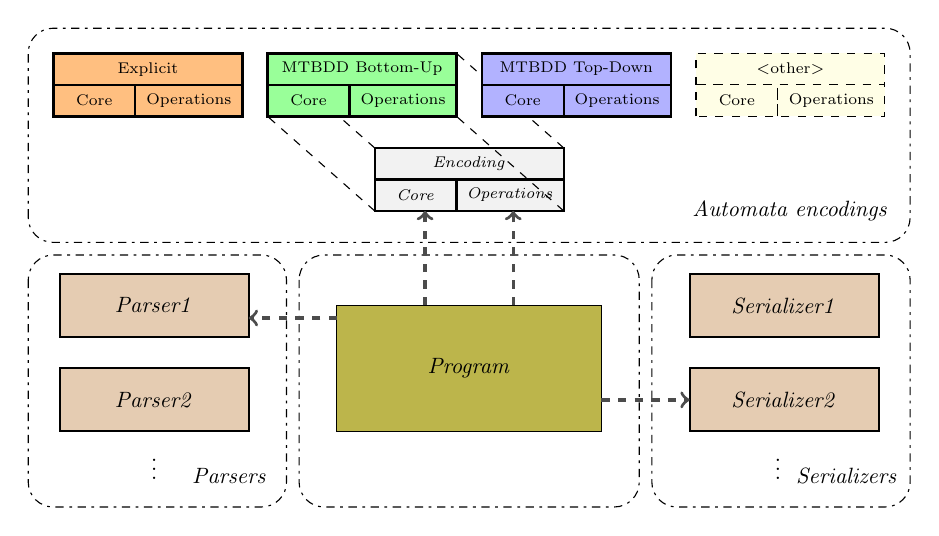
\begin{tikzpicture}
[
  scale=1,
  transform shape,
	gen/.style={thick,fill=gray!10},
	expl/.style={thick,fill=orange!50},
	bu/.style={thick,fill=green!40},
	td/.style={thick,fill=blue!30},
	other/.style={fill=yellow!10,dashed}
]

% encodings
\draw[dashed] (0,1) -- (-1.7,2.5);
\draw[dashed] (0,0) -- (-1.7,1.5);
\draw[dashed] (3,1) -- (1.3,2.5);

\draw (0,0.5) rectangle +(3, 0.5) [gen] node[midway] {\textit{\scriptsize{Encoding}}};
\draw (0,0) rectangle +(1.3, 0.5) [gen] node[midway] {\textit{\scriptsize{Core}}};
\draw (1.3,0) rectangle +(1.7, 0.5) [gen] node[midway] {\textit{\scriptsize{Operations}}};

\draw (-5.1,2) rectangle +(3, 0.5) [expl] node[midway] {\scriptsize{Explicit}};
\draw (-5.1,1.5) rectangle +(1.3, 0.5) [expl] node[midway] {\scriptsize{Core}};
\draw (-3.8,1.5) rectangle +(1.7, 0.5) [expl] node[midway] {\scriptsize{Operations}};

\draw (-1.7,2) rectangle +(3, 0.5) [bu] node[midway] {\scriptsize{MTBDD Bottom-Up}};
\draw (-1.7,1.5) rectangle +(1.3, 0.5) [bu] node[midway] {\scriptsize{Core}};
\draw (-0.4,1.5) rectangle +(1.7, 0.5) [bu] node[midway] {\scriptsize{Operations}};

\draw (1.7,2) rectangle +(3, 0.5) [td] node[midway] {\scriptsize{MTBDD Top-Down}};
\draw (1.7,1.5) rectangle +(1.3, 0.5) [td] node[midway] {\scriptsize{Core}};
\draw (3.0,1.5) rectangle +(1.7, 0.5) [td] node[midway] {\scriptsize{Operations}};

\draw (5.1,2) rectangle +(3, 0.5) [other] node[midway] {\scriptsize{$<$other$>$}};
\draw (5.1,1.5) rectangle +(1.3, 0.5) [other] node[midway] {\scriptsize{Core}};
\draw (6.4,1.5) rectangle +(1.7, 0.5) [other] node[midway] {\scriptsize{Operations}};

\draw[dashed] (3,0) -- (1.3,1.5);

\draw[rounded corners=9,dash pattern=on 3pt off 2pt on 1pt off 2pt] (-5.5,-0.5) rectangle +(14,3.4);

\draw (6.6,0) node {\textit{Automata encodings}};


% parsers
\draw (-5,-2) rectangle +(3, 1) [gen,fill=brown!40] node[midway] (parser1) {\textit{Parser1}};
\draw (-5,-3.5) rectangle +(3, 1) [gen,fill=brown!40] node[midway] {\textit{Parser2}};
\draw (-3.5,-4) node {$\vdots$};

\draw[rounded corners=9,dash pattern=on 3pt off 2pt on 1pt off 2pt] (-5.5,-0.7) rectangle +(4.1,-4);
\draw (-2.3,-4.2) node {\textit{Parsers}};

% serializers
\draw (5,-2) rectangle +(3, 1) [gen,fill=brown!40] node[midway] {\textit{Serializer1}};
\draw (5,-3.5) rectangle +(3, 1) [gen,fill=brown!40] node[midway] {\textit{Serializer2}};
\draw (6.4,-4) node {$\vdots$};

\draw[rounded corners=9,dash pattern=on 3pt off 2pt on 1pt off 2pt] (4.4,-0.7) rectangle +(4.1,-4);
\draw (7.5,-4.2) node {\textit{Serializers}};

% program
\draw[rounded corners=9,dash pattern=on 3pt off 2pt on 1pt off 2pt] (-1.2,-0.7) rectangle +(5.4,-4);

\draw[fill=olive!60] (-0.6,-1.5) rectangle (3.6,-3.5) node[midway] {\textit{Program}};

\draw[very thick,dashed,->,black!70] (-0.6,-1.7) -- (-2,-1.7);
\draw[very thick,dashed,->,black!70] (3.6,-3) -- (5,-3);
\draw[very thick,dashed,->,black!70] (0.8,-1.5) -- (0.8,0);
\draw[very thick,dashed,->,black!70] (2.2,-1.5) -- (2.2,0);

\end{tikzpicture}

		\caption{The main concept of \vata. Figure is taken from \cite{tacas12}}.
		\label{fig:vata}
\end{center}
\end{figure}

A \emph{program} (e.g. cli of VATA is such a program) employing the three parts of \vata\ could works as follows.
An input automaton is loaded by one of the parsers to an intermediate representation.
The wrapping program chooses internal encoding of NTA to which is automaton stored from intermediate encoding (please note that it is also
create automaton in the chosen enconding directly using API provided by VATA).
Then the automaton is processed and the applied operations are implemented by module of the chosen encoding.
Finally, automaton could be serialized to an output format.
When one wants to add her own encoding then she needs to implement only core of encoding (with API for creating automaton itself)
and ofcourse needed operations and can employ already implemented parses and serializers of \vata.

\subsection{Implemented NTA encodings}

Using \emph{explicit enconding} NTA transition relation is represented by a hiearchy of the hash tables as it is shown in Figure \ref{fig:explnta}.
The first level of the hash tables hiearchy (\emph{top-level lookup tables}) maps each state $q$ of an automaton to 
a second level of the hash tables hiearchy (\emph{transition cluster}) where are store all symbols which
are presented in a transition where $q$ is at left-handed side.
Each symbol $a$ in a transition cluster is mapped to a pointer to a set in the third level of hiearchy (\emph{sets of pointers to tuples}).
The set contains pointers to tuples which are at right-handed side in a transition with $q$ at left-handed side and with $a$ as a symbol.
The tuples are stored at a special set where every tuples is stored only once.
Please note, that it also possible to share part of transition relation between different automata what
brings higher efficiency in space complexity of implementation.
Module for explicit encoding also stores explicitly set of the final states of a NFA but on
the other side it does not store anywhere explicitly set of states because it can be obtained from a transition relation.

\begin{figure}[bt]
\begin{center}
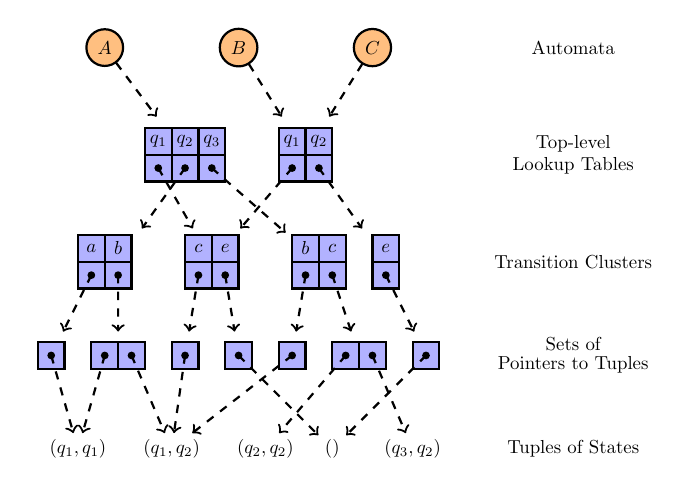
\begin{tikzpicture}
[
  scale=0.85,
  transform shape,
	gen/.style={thick,fill=gray!10},
	expl/.style={thick,fill=orange!50},
	bu/.style={thick,fill=green!40},
	td/.style={thick,fill=blue!30},
	other/.style={fill=yellow!10,dashed}
]

\node at(10,2) {Automata};

\node[expl,circle,draw] (aA) at(1.25,2) {\textit{$A$}};
\node[expl,circle,draw] (aB) at(3.75,2) {\textit{$B$}};
\node[expl,circle,draw] (aC) at(6.25,2) {\textit{$C$}};


\node at(10,0) {\shortstack{Top-level\\ Lookup Tables}};

\node[minimum size=40pt](table1) at (2.75,0) {};
\draw (2,0) rectangle +(0.5, .5) [td] node[midway] {\textit{$q_1$}};
\draw (2,-.5) rectangle +(0.5, .5) [td] node[midway] {};
\draw (2.5,0) rectangle +(0.5, .5) [td] node[midway] {\textit{$q_2$}};
\draw (2.5,-.5) rectangle +(0.5, .5) [td] node[midway] {};
\draw (3,0) rectangle +(0.5, .5) [td] node[midway] {\textit{$q_3$}};
\draw (3,-.5) rectangle +(0.5, .5) [td] node[midway] {};

\node[minimum size=40pt](table2) at (5,0) {};
\draw (4.5,0) rectangle +(0.5, .5) [td] node[midway] {\textit{$q_1$}};
\draw (4.5,-.5) rectangle +(0.5, .5) [td] node[midway] {};
\draw (5,0) rectangle +(0.5, .5) [td] node[midway] {\textit{$q_2$}};
\draw (5,-.5) rectangle +(0.5, .5) [td] node[midway] {};


\draw[->,thick,dashed] (aA) -- (table1);
\draw[->,thick,dashed] (aB) -- (table2);
\draw[->,thick,dashed] (aC) -- (table2);


\node at(10,-2) {Transition Clusters};

\node[minimum size=35](cluster1) at (1.5,-2) {};
\draw (0.75,-2) rectangle +(0.5, .5) [td] node[midway] {\textit{$a$}};
\draw (0.75,-2.5) rectangle +(0.5, .5) [td] node[midway] {};
\draw (1.25,-2) rectangle +(0.5, .5) [td] node[midway] {\textit{$b$}};
\draw (1.25,-2.5) rectangle +(0.5, .5) [td] node[midway] {};

\node[minimum size=35pt](cluster2) at (3.25,-2) {};
\draw (2.75,-2) rectangle +(0.5, .5) [td] node[midway] {\textit{$c$}};
\draw (2.75,-2.5) rectangle +(0.5, .5) [td] node[midway] {};
\draw (3.25,-2) rectangle +(0.5, .5) [td] node[midway] {\textit{$e$}};
\draw (3.25,-2.5) rectangle +(0.5, .5) [td] node[midway] {};

\node[minimum size=35pt](cluster3) at (5.25,-2) {};
\draw (4.75,-2) rectangle +(0.5, .5) [td] node[midway] {\textit{$b$}};
\draw (4.75,-2.5) rectangle +(0.5, .5) [td] node[midway] {};
\draw (5.25,-2) rectangle +(0.5, .5) [td] node[midway] {\textit{$c$}};
\draw (5.25,-2.5) rectangle +(0.5, .5) [td] node[midway] {};

\node[minimum size=35pt](cluster4) at (6.5,-2) {};
\draw (6.25,-2) rectangle +(0.5, .5) [td] node[midway] {\textit{$e$}};
\draw (6.25,-2.5) rectangle +(0.5, .5) [td] node[midway] {};


\draw[thick,fill=black] (2.25,-0.25) circle (0.5mm);
\draw[->,thick,dashed] (2.25,-.25) -- (cluster2);

\draw[thick,fill=black] (2.75,-0.25) circle (0.5mm);
\draw[->,thick,dashed] (2.75,-.25) -- (cluster1);

\draw[thick,fill=black] (3.25,-0.25) circle (0.5mm);
\draw[->,thick,dashed] (3.25,-.25) -- (cluster3);

\draw[thick,fill=black] (4.75,-0.25) circle (0.5mm);
\draw[->,thick,dashed] (4.75,-.25) -- (cluster2);

\draw[thick,fill=black] (5.25,-0.25) circle (0.5mm);
\draw[->,thick,dashed] (5.25,-.25) -- (cluster4);


\node at(10,-3.75) {\shortstack{Sets of\\ Pointers to Tuples}};

\node[minimum size=25pt](set1) at (0.25,-3.75) {};
\draw (0,-4) rectangle +(0.5, .5) [td] node[midway] {};

\node[minimum size=25pt](set2) at (1.5,-3.75) {};
\draw (1,-4) rectangle +(0.5, .5) [td] node[midway] {};
\draw (1.5,-4) rectangle +(0.5, .5) [td] node[midway] {};

\node[minimum size=25pt](set3) at (2.75,-3.75) {};
\draw (2.5,-4) rectangle +(0.5, .5) [td] node[midway] {};

\node[minimum size=25pt](set4) at (3.75,-3.75) {};
\draw (3.5,-4) rectangle +(0.5, .5) [td] node[midway] {};

\node[minimum size=25pt](set5) at (4.75,-3.75) {};
\draw (4.5,-4) rectangle +(0.5, .5) [td] node[midway] {};

\node[minimum size=25pt](set6) at (6,-3.75) {};
\draw (5.5,-4) rectangle +(0.5, .5) [td] node[midway] {};
\draw (6,-4) rectangle +(0.5, .5) [td] node[midway] {};

\node[minimum size=25pt](set7) at (7.25,-3.75) {};
\draw (7,-4) rectangle +(0.5, .5) [td] node[midway] {};


\draw[thick,fill=black] (1,-2.25) circle (0.5mm);
\draw[->,thick,dashed] (1,-2.25) -- (set1);

\draw[thick,fill=black] (1.5,-2.25) circle (0.5mm);
\draw[->,thick,dashed] (1.5,-2.25) -- (set2);

\draw[thick,fill=black] (3,-2.25) circle (0.5mm);
\draw[->,thick,dashed] (3,-2.25) -- (set3);

\draw[thick,fill=black] (3.5,-2.25) circle (0.5mm);
\draw[->,thick,dashed] (3.5,-2.25) -- (set4);

\draw[thick,fill=black] (5,-2.25) circle (0.5mm);
\draw[->,thick,dashed] (5,-2.25) -- (set5);

\draw[thick,fill=black] (5.5,-2.25) circle (0.5mm);
\draw[->,thick,dashed] (5.5,-2.25) -- (set6);

\draw[thick,fill=black] (6.5,-2.25) circle (0.5mm);
\draw[->,thick,dashed] (6.5,-2.25) -- (set7);


\node at(10,-5.5) {Tuples of States};

\node(tup1) at (0.75,-5.5) {$(q_1, q_1)$};
\node(tup2) at (2.5,-5.5) {$(q_1, q_2)$};
\node(tup3) at (4.25,-5.5) {$(q_2, q_2)$};
\node(tup4) at (7,-5.5) {$(q_3, q_2)$};
\node(tup5) at (5.5,-5.5) {$()$};

\draw[thick,fill=black] (0.25,-3.75) circle (0.5mm);
\draw[->,thick,dashed] (0.25,-3.75) -- (tup1);

\draw[thick,fill=black] (1.25,-3.75) circle (0.5mm);
\draw[->,thick,dashed] (1.25,-3.75) -- (tup1);

\draw[thick,fill=black] (1.75,-3.75) circle (0.5mm);
\draw[->,thick,dashed] (1.75,-3.75) -- (tup2);

\draw[thick,fill=black] (2.75,-3.75) circle (0.5mm);
\draw[->,thick,dashed] (2.75,-3.75) -- (tup2);

\draw[thick,fill=black] (3.75,-3.75) circle (0.5mm);
\draw[->,thick,dashed] (3.75,-3.75) -- (tup5);

\draw[thick,fill=black] (4.75,-3.75) circle (0.5mm);
\draw[->,thick,dashed] (4.75,-3.75) -- (tup2);

\draw[thick,fill=black] (5.75,-3.75) circle (0.5mm);
\draw[->,thick,dashed] (5.75,-3.75) -- (tup3);

\draw[thick,fill=black] (6.25,-3.75) circle (0.5mm);
\draw[->,thick,dashed] (6.25,-3.75) -- (tup4);

\draw[thick,fill=black] (7.25,-3.75) circle (0.5mm);
\draw[->,thick,dashed] (7.25,-3.75) -- (tup5);


\end{tikzpicture}

	\caption{Explicit representation of NTA by \vata. Figure is taken from \cite{tacas12}}.
	\label{fig:explnta}
\end{center}
\end{figure}

\begingroup
\tikzset{every picture/.style={scale=0.8}}%
\begin{figure}[bt]
\label{fig:symnta}
	\centering
	\begin{subfigure}{.5\textwidth}
		\centering
		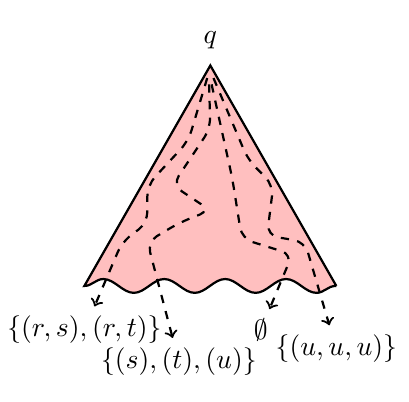
\begin{tikzpicture}
[]
\useasboundingbox (-2.9,-4.9) rectangle (2.7,0.6);

<<<<<<< HEAD
=======

>>>>>>> fcad047018e021c44f6be41eab656d5ec3da0ca5
%\draw[thick,fill=blue!40] (3,-5) -- (0,0) -- (-3,-5) .. controls (-1,-3.5) and (1,-6.5) .. (3,-5);
\draw[thick,fill=pink] (2,-3.5) -- (0,0) -- (-2,-3.5) decorate[decoration=snake,segment length=22] { -- cycle};

\node at (0,0.4){$q$};

\node(set1) at (-2,-4.2) {$\{(r,s),(r, t)\}$};
\node(set2) at (-0.5,-4.7) {$\{(s), (t), (u)\}$};
\node(set3) at (0.8,-4.2) {$\emptyset$};
\node(set4) at (2,-4.5) {$\{(u, u, u)\}$};

\draw[->,thick,dashed,rounded corners] (-0.05,-0.2) -- (-0.35,-1.2) -- (-1,-1.9) -- (-1,-2.5) -- (-1.4,-2.8) -- (set1);
\draw[->,thick,dashed,rounded corners] (-0.02,-0.3) -- (0,-1) -- (-0.6,-1.9) -- (0,-2.3) -- (-0.5,-2.5) -- (-1,-2.8) -- (set2);
\draw[->,thick,dashed,rounded corners] (0.02,-0.3) -- (0.35,-1.8) -- (0.5,-2.75) -- (1.3,-3) -- (set3);
\draw[->,thick,dashed,rounded corners] (0.05,-0.2) -- (0.6,-1.5) -- (1,-1.9) -- (0.9,-2.7) -- (1.5,-2.8) -- (set4);



\end{tikzpicture}
		\caption{MTBDD Top-down representation of a NTA. Image is taken from \cite{tacas12}.}
		\label{fig:mtbdd_td}
	\end{subfigure}%
	~
	\begin{subfigure}{.5\textwidth}
	\centering
	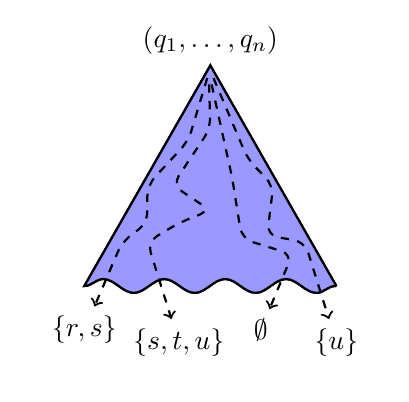
\begin{tikzpicture}
[]
\useasboundingbox (-2.9,-4.9) rectangle (2.7,0.6);
<<<<<<< HEAD
%\draw[thick,fill=blue!40] (3,-5) -- (0,0) -- (-3,-5) .. controls (-1,-3.5) and (1,-6.5) .. (3,-5);
\draw[thick,fill=blue!40] (2,-3.5) -- (0,0) -- (-2,-3.5) decorate[decoration=snake,segment length=22] { -- cycle};

=======

%\draw[thick,fill=blue!40] (3,-5) -- (0,0) -- (-3,-5) .. controls (-1,-3.5) and (1,-6.5) .. (3,-5);
\draw[thick,fill=blue!40] (2,-3.5) -- (0,0) -- (-2,-3.5) decorate[decoration=snake,segment length=22] { -- cycle};


>>>>>>> fcad047018e021c44f6be41eab656d5ec3da0ca5
\node at (0,0.4){$(q_1,\dots, q_n)$};

\node(set1) at (-2,-4.2) {$\{r,s\}$};
\node(set2) at (-0.5,-4.4) {$\{s, t, u\}$};
\node(set3) at (0.8,-4.2) {$\emptyset$};
\node(set4) at (2,-4.4) {$\{u\}$};

\draw[->,thick,dashed,rounded corners] (-0.05,-0.2) -- (-0.35,-1.2) -- (-1,-1.9) -- (-1,-2.5) -- (-1.4,-2.8) -- (set1);
\draw[->,thick,dashed,rounded corners] (-0.02,-0.3) -- (0,-1) -- (-0.6,-1.9) -- (0,-2.3) -- (-0.5,-2.5) -- (-1,-2.8) -- (set2);
\draw[->,thick,dashed,rounded corners] (0.02,-0.3) -- (0.35,-1.8) -- (0.5,-2.75) -- (1.3,-3) -- (set3);
\draw[->,thick,dashed,rounded corners] (0.05,-0.2) -- (0.6,-1.5) -- (1,-1.9) -- (0.9,-2.7) -- (1.5,-2.8) -- (set4);



\end{tikzpicture}
	\caption{MTBDD Bottom-up representation of a NTA. Image is taken from \cite{tacas12}.}
	\label{fig:mtbdd_bu}
	\end{subfigure}%
\end{figure}
\endgroup

Another already implemented encoding is semi-symbolic based on VATA own implementation of MTBDD package.
Because semi-symblic encoding and MTBDD are not in the aim of this thesis the will no be detaily described
but it is possbile to find such kind of description in \cite{lengal10}.
The main idea of semi-symbolic encoding is shown in Figure \ref{fig:symnta}.
First of all it is necessary to distinguish between (a) top-down and (b) bottom-up variants of this encoding.
The first one maps each state $q$ of a NTA using MTBDD to the sets of the tuples of states such that that it is possible
to make transtion from $q$ under a symbol $a$ to a tuple in apropriate set (each set of tuples is dedicated
to one symbol under which it is possible to make transition from $q$ to the tuples in the set).
The former one symetrically maps each n-tuple $(q_1,\ldots,q_n)$ of a NFA using MTBDD to the sets of states
where each set $S$ is dedicated to a symbol $a$ of the NFA and contains states such that there exists a transition
with $(q_1,\ldots,q_n)$ on the right-handed side and symbol $a$ and state from the set $S$ on the left-handed side.
The final state set of a NTA is again represented by explicit set in both variants,
state set is not stored explicitly because one can obtain it from transition relation and
the symbols are encoded in MTBDD.

All of the mentioned encodings currently support efficient language inclusion checking using algorithm
from \cite{tacas10} but this does not hold for other operations because some of them are not implemented yet for specific encoding.
The full enumeration of the supported operations for the particular encodings is given in Table \ref{tab:vataop}.

\begin{table}[bt]
	\begin{center}
		\catcode`\-=12
		\begin{tabular}{| l | c | c | c |} \hline
		& {\textbf{Explicit}} & \multicolumn{2}{|c|}{\textbf{Semi-symbolic}} \\ \cline{2-4}
		\textbf{Operation} & \textbf{top-down} & \textbf{bottom-up} & \textbf{top-down} \\ \hline
		Union & $+$ & $+$ & $+$ \\
		Intersection & $+$ & $+$ & $+$ \\
		Complement (experimental) & $+$ & $+$ & $+$ \\
		Removing useless states & $+$ & $+$ & $+$ \\
		Removing unreachable states & $+$ & $+$ & $+$ \\
		Simulation & $+$ & $-$ & $-$ \\
		Downward Inclusion  & $+$ & $+$ & $-$ \\ 
		Upward Inclusion  & $+$ & $-$ & $-$ \\ 
		Simulation over LTS (Labeled Transitions System) & $+$ & $-$ & $-$ \\ \hline
		\end{tabular}
	\caption{Table of supported operations over NTA by particular encodings implemented in \vata.
	Table is taken from \cite{hruska13}.}
	\label{tab:vataop}
	\end{center}
\end{table}


\section{The Forester Tool}
\label{sec:FA}


\section{Forester with VATA}
\label{sec:fova}

\subsection{Adapter design pattern}

\chapter{??Predicate Abstraction and Backward Run??}
\label{ch:pred}

\chapter{Backward Run in Forest Automata Based Verification}
\label{ch:backward}

\section{Backward Run over Symbolic Context}

\section{Intersection of Forest Automata}

\chapter{Implementation}
\label{ch:impl}

\section{Execution Trace}
\section{Module For Intersection}

\chapter{Evaluation}
\label{ch:eval}

\chapter{Conclusion}
\label{ch:concl}
